\documentclass[12pt,a4paper]{article}
\usepackage{fontspec}
\usepackage{polyglossia}
\setdefaultlanguage{russian}
\setmainfont{STIX Two Text}[AutoFakeBold=1.5]
\setmonofont{Menlo}
\newfontfamily\cyrillicfonttt{Menlo}
\usepackage[a4paper,margin=2cm]{geometry}
\usepackage{graphicx,longtable,tabularx,array,booktabs}
\usepackage{float,caption,enumitem,pdflscape,xurl,listings,tikz}
\usepackage{hyperref,etoolbox}
\usetikzlibrary{positioning,arrows.meta}
\hypersetup{colorlinks=true,linkcolor=blue,urlcolor=blue}
\lstset{basicstyle=\ttfamily\footnotesize,breaklines=true,columns=fullflexible,frame=single,keepspaces=true,showstringspaces=false}
\setlength{\parindent}{1.25cm}
\setlength{\parskip}{0.25em}
\renewcommand{\arraystretch}{1.16}
\setlist{nosep,leftmargin=1.5em}
\AtBeginEnvironment{longtable}{\small}
\sloppy
\begin{document}
\begin{titlepage}
\centering
{\large Практическая работа\par}
\vspace{2.2cm}
{\LARGE\bfseries Отчёт по практической работе № 6\par}
\vspace{0.6cm}
{\Large Предотвращение инъекций и ошибок работы с файлами\par}
\vspace{1.8cm}
\begin{tabular}{p{4cm}p{11cm}}
Дисциплина: & Основы разработки защищённого программного обеспечения и компьютерных сетей\\
Вариант: & 19 — Система учёта транспортных средств организации\\
Исходная версия: & v0.5\\
Версия работы: & v0.6\\
Студент: & Мостовая Полина Андреевна\\
Группа: & ИУСбд-02-23
\end{tabular}
\vfill
{\large 2026\par}
\end{titlepage}
\tableofcontents
\clearpage

\section{Тема, цель и характеристика проекта}
Цель работы — безопасно использовать проверенные в ЛР №5 данные при работе с SQLite и файловой системой, исследовать передачу аргументов процессу и проверить компоненты автоматизированными позитивными и негативными тестами \cite{guide6}. Работа продолжает v0.5. Исходный валидатор проекта называется \texttt{validate\_request()}, поэтому интеграция сохраняет его фактический API.

Прототип не является веб-сервисом: в нём нет сетевого API, входа пользователей и авторизации заявок. ЛР6 добавляет локальную модель обращения, SQLite-репозиторий, каталог вложений и демонстрацию. Это не означает, что все функции учета автопарка и поездок уже реализованы.

\section{Архитектура}
На входе \texttt{validate\_request} ограничивает и проверяет JSON и создаёт неизменяемый \texttt{ValidatedRequest}. \texttt{RequestService} связывает SQLite и FileStore: сначала сохраняется проверенное вложение, затем строка БД; при ошибке INSERT предпринимается удаление файла.
\begin{figure}[H]
\centering
\resizebox{\textwidth}{!}{%
\begin{tikzpicture}[node distance=8mm and 11mm,box/.style={draw,rounded corners,align=center,text width=3.1cm,minimum height=11mm,font=\scriptsize},arrow/.style={-{Stealth},thick}]
\node[box] (input) {Недоверенные JSON и байты};
\node[box,right=of input] (valid) {\shortstack{Проверка JSON\\\texttt{ValidatedRequest}}};
\node[box,right=of valid] (service) {\shortstack{Сервис заявок\\\texttt{RequestService}}};
\node[box,above right=of service] (repo) {\shortstack{SQLite-репозиторий\\\texttt{RequestRepository}}};
\node[box,below right=of service] (store) {\shortstack{Хранилище\\\texttt{FileStore}}};
\node[box,right=of repo] (sqlite) {SQLite};
\node[box,right=of store] (fs) {Каталог 0700};
\draw[arrow] (input) -- (valid);
\draw[arrow] (valid) -- (service);
\draw[arrow] (service) -- (repo);
\draw[arrow] (service) -- (store);
\draw[arrow] (repo) -- (sqlite);
\draw[arrow] (store) -- (fs);
\draw[arrow,dashed] (repo.south) to[bend right=22] node[below,font=\scriptsize,align=center]{ошибка записи: удалить файл} (store.north);
\end{tikzpicture}
}
\caption{Компоненты и компенсирующее действие при ошибке SQLite.}
\end{figure}

\section{Безопасный SQLite Repository}
\texttt{RequestRepository} использует стандартный модуль \texttt{sqlite3}. Операции добавления, чтения, изменения приоритета и удаления передают значения через параметры \texttt{?}. Сортировка является единственным динамическим SQL-фрагментом и выбирается из констант \texttt{newest} и \texttt{priority}; пользовательский текст никогда не попадает в него. Маркеры параметров предназначены для значений, а не имён колонок или SQL-операторов \cite{pythonSqlite,owaspSql,cwe89}.

Таблица задаёт первичный ключ, обязательность и диапазоны полей через \texttt{NOT NULL}/\texttt{CHECK}; \texttt{file\_id} уникален. Для пары вложения установлено соответствие: оба поля отсутствуют или оба присутствуют, а ID состоит ровно из 32 строчных шестнадцатеричных символов. \texttt{delete\_unattached} использует условный \texttt{DELETE ... AND file\_id IS NULL}, поэтому строка с вложением не удаляется.

\section{FileStore и политика файлов}
\texttt{FileStore} принимает только логический тип вложения и bytes; физический путь от пользователя не принимается. ID формируется через \texttt{secrets.token\_hex(16)}. Размер ограничен 1\,048\,576 байт. Создание использует \texttt{O\_CREAT | O\_EXCL}; файл получает права 0600, каталог хранилища — 0700. Чтение ограничено пределом \texttt{MAX\_BYTES + 1}, проверяет открытый дескриптор через \texttt{fstat} и требует обычный файл.

Политика типов: \texttt{log} — строгий UTF-8 без NUL; \texttt{report} — начальная сигнатура \texttt{\%PDF-}; \texttt{screenshot} и вариант 19 \texttt{vehicle\_photo} — 8-байтовая PNG-сигнатура. Это первичная фильтрация, не полная проверка PDF/изображения, не антивирусный анализ и не гарантия безопасного рендеринга. JPEG для \texttt{vehicle\_photo} не поддерживается.

\section{Индивидуальное задание №19: символические ссылки}
Каталог открывается с \texttt{O\_DIRECTORY | O\_NOFOLLOW}; создание, чтение и удаление выполняются относительно дескриптора каталога через \texttt{dir\_fd}. Файл открывается с \texttt{O\_NOFOLLOW}; после открытия тип объекта устанавливается по \texttt{fstat}. Такая последовательность избегает отдельной проверки пути перед открытием и уменьшает окно TOCTOU и выхода по traversal-пути \cite{pythonOs,cwe22,cwe367}. Вызовы и доступность флагов платформозависимы, поэтому при отсутствии необходимых функций хранилище отказывает закрытым образом.

Выполнены три отдельные проверки: (1) ID указывает на ссылку на внешний файл — чтение отклонено; (2) случайно выбранное имя уже является ссылкой — \texttt{O\_EXCL} не позволяет открыть цель и генератор повторяет попытку; внешний целевой файл не изменяется; (3) корневой каталог после инициализации заменяется ссылкой — операция отказывает. Эти результаты относятся к текущей ОС и не доказывают защиту от администратора ОС, компрометации процесса или небезопасного родительского каталога.

\section{Командная инъекция и аргументы процесса}
Для CRUD и файловых операций внешняя команда не нужна. Отдельная учебная функция \texttt{safe\_argument} использует фиксированный исполняемый Python, список аргументов, \texttt{shell=False}, таймаут 5 секунд и максимальную длину 200 символов. Тест передает \texttt{example; echo TEST}: строка возвращается как один аргумент, команда оболочки не запускается. \texttt{shell=False} разделяет команду и аргументы, но программа-цель может трактовать аргумент как опцию или путь; поэтому проверка аргументов всё ещё обязательна \cite{owaspCommand,cwe78}.

\section{Таблица тестовых сценариев}
Обязательные 15 ситуаций методички отражены в тестах ниже. Дополнительно тестируются точные типы, ограничение ID, варианты 19 и интеграция. Полный набор проекта на текущем первом проходе: \textbf{120 passed, 9 subtests passed} по команде \texttt{./.venv/bin/python -m pytest -q}. Повторный запуск полного набора зафиксирован на скриншоте.
\small
\begin{longtable}{p{0.65cm}p{7.2cm}p{4.35cm}p{1.9cm}}
\caption{Базовые сценарии методички и текущие результаты}\\
\toprule № & Сценарий & Ожидаемый результат / тест & Статус\\ \midrule\endfirsthead
\toprule № & Сценарий & Ожидаемый результат / тест & Статус\\ \midrule\endhead
1 & Создание и чтение заявки & Сохранение и чтение полей & Пройдено\\
2 & Изменение приоритета & Обновлённое значение & Пройдено\\
3 & Удаление без вложения & Запись удалена & Пройдено\\
4 & SQL-подобный текст & Сохранён как обычное значение & Пройдено\\
5 & Неизвестная сортировка & Контролируемый отказ & Пройдено\\
6 & Неизвестная категория & Контролируемый отказ & Пройдено\\
7 & Булев приоритет & Отклонён & Пройдено\\
8 & LIMIT вне диапазона & Отклонён & Пройдено\\
9 & Сохранение и чтение файла & Байты совпадают & Пройдено\\
10 & Превышение 1 МиБ & Отклонено & Пройдено\\
11 & Неизвестный тип файла & Отклонён & Пройдено\\
12 & Неверная сигнатура PDF & Отклонена & Пройдено\\
13 & Path Traversal через ID & Отклонён & Пройдено\\
14 & Некорректный UTF-8 log & Отклонён & Пройдено\\
15 & Ошибка SQLite & Файл удалён компенсацией & Пройдено\\
\bottomrule
\end{longtable}
\normalsize

Вариант 19 проверен тремя тестами (внешняя symlink при чтении; коллизия symlink при создании; замена корня symlink). Отдельно проверено сохранение \texttt{vehicle\_photo} с PNG-сигнатурой, отказ JPEG-подобной сигнатуры и сквозная запись ключа в SQLite. Автотесты вызываются через \texttt{tests/test\_v06.py}.

\section{Интеграционная демонстрация}
Команда \texttt{python demo\_v06.py} проверяет JSON функцией \texttt{validate\_request}, создаёт временную SQLite-БД и FileStore, сохраняет заявку с журналом, читает его и сравнивает байты, а затем демонстрирует передачу аргумента. Временный каталог удаляется при завершении. Результат демонстрации зафиксирован на скриншоте вместе с полным запуском тестов.

\section{Ограничения и остаточные риски}
Компенсационное удаление не образует общей транзакции файловой системы и SQLite; сбой удаления может оставить файл, а аварийное завершение процесса может произойти между двумя шагами. Права каталога и его родителей должны исключать запись посторонних процессов. \texttt{O\_NOFOLLOW}, \texttt{O\_DIRECTORY} и \texttt{dir\_fd} доступны не на каждой ОС; реализация отказывает, если безопасное открытие недоступно. Проверка сигнатуры не разбирает файлы полностью. SQLite-файл является локальным хранилищем без настроенной аутентификации/авторизации и без политики резервирования. Тесты подтверждают только проверенные сценарии текущего прототипа.

\section{Вывод}
В v0.6 добавлены параметризованный Repository, ограниченный FileStore и сервис, связывающий проверенное обращение с вложением. Вариант 19 проверен отдельными сценариями symlink; ключ \texttt{vehicle\_photo} из v0.5 сохранён, для него определена PNG-сигнатура. На приложенных снимках показаны вывод демонстрации, полный запуск тестов и три проверки варианта 19.

\section{Скриншоты демонстрации и проверок}
\begin{figure}[H]
\centering
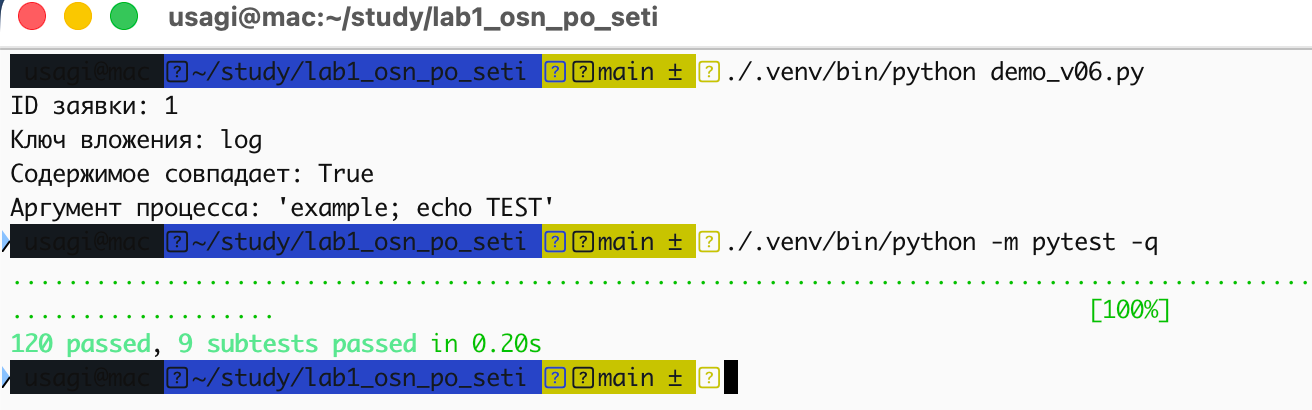
\includegraphics[width=.98\textwidth,height=.7\textheight,keepaspectratio]{screenshots_manual/lab6_demo_tests.png}
\caption{Вывод сквозной демонстрации и полный запуск тестового набора v0.6.}
\end{figure}
\begin{figure}[H]
\centering
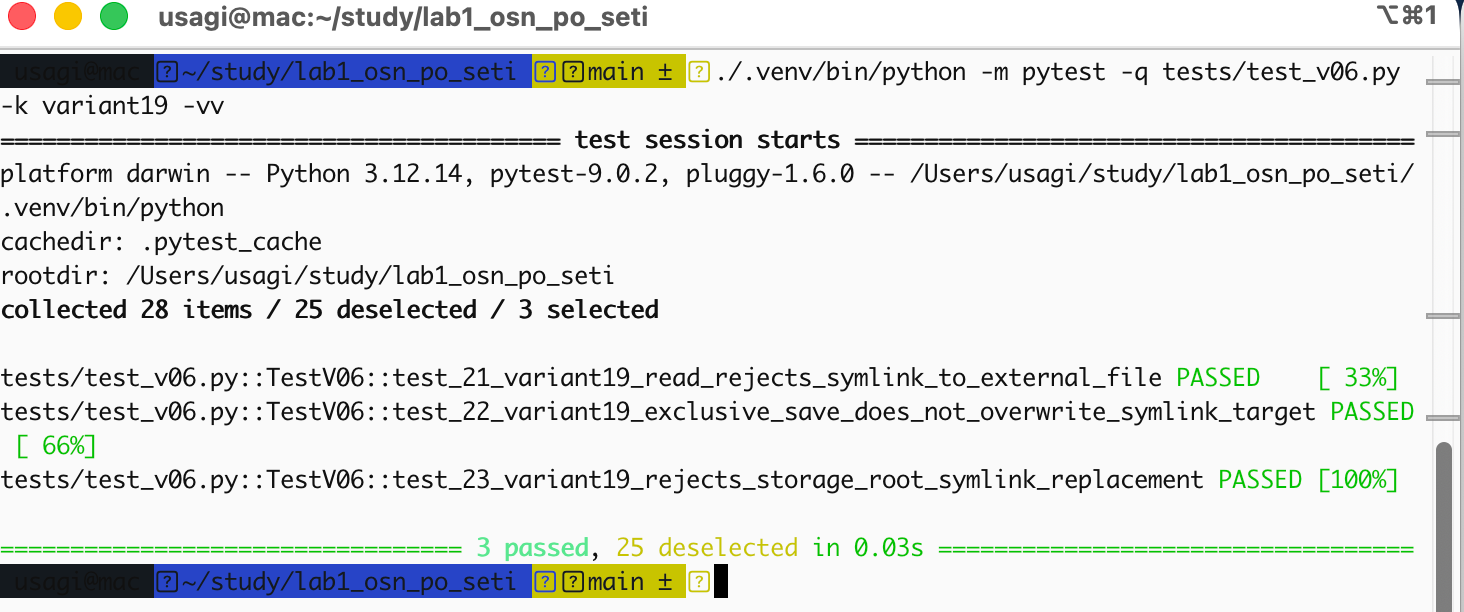
\includegraphics[width=.98\textwidth,height=.7\textheight,keepaspectratio]{screenshots_manual/lab6_symlink.png}
\caption{Три пройденные проверки защиты варианта 19 от symlink.}
\end{figure}

\section{Ответы на контрольные вопросы}
\begin{enumerate}
\item SQL-инъекция — изменение структуры или смысла SQL внешними данными.
\item Она возникает, когда данные конкатенируют с SQL-текстом вместо передачи отдельно.
\item Параметризованный запрос отделяет команду SQL от значений и связывает их через маркеры.
\item f-строка формирует SQL-текст до вызова драйвера; специальные значения могут превратиться в операторы SQL.
\item Allowlist — фиксированный перечень разрешённых значений, из которого приложение выбирает режим.
\item Repository Layer изолирует операции хранения и их правила от сервисной логики.
\item CRUD — Create, Read, Update, Delete: создать, прочитать, изменить, удалить.
\item Path Traversal — использование пути для выхода за пределы назначенного каталога.
\item Абсолютный путь задаётся от корня файловой системы; относительный — от базового/текущего каталога.
\item TOCTOU — гонка между проверкой ресурса и его использованием, когда состояние ресурса может измениться.
\item \texttt{O\_EXCL} совместно с \texttt{O\_CREAT} запрещает создание, если имя уже существует.
\item \texttt{O\_NOFOLLOW} запрещает следовать по конечному компоненту, если это symlink, на ОС с поддержкой флага.
\item Физическое имя позволяет управлять путём, провоцировать traversal и коллизии; внутренний ID отделяет интерфейс от пути.
\item Лимит ограничивает расход памяти, диска и ресурсов последующей обработки.
\item Сигнатура — лишь ограниченный признак формата; она не подтверждает целостность, безопасную структуру или отсутствие активного содержимого.
\item OS Command Injection — изменение команды или её интерпретации через внешнее значение.
\item При \texttt{shell=True} строка разбирается оболочкой; метасимволы могут стать операторами и запустить дополнительные команды.
\item Внедрение аргумента меняет параметры заданной программы; командная инъекция меняет выполняемую команду. Опция может быть опасна и без оболочки.
\item Компенсирующая операция пытается отдельно обратить ранее выполненный шаг после сбоя следующего шага.
\item Файловая система и SQLite не участвуют в общей транзакции; авария или отказ удаления может помешать компенсации.
\item Негативные тесты проверяют, что ошибочные и вредоносно сформированные входы приводят к контролируемому отказу.
\item Успешные тесты подтверждают лишь выбранные сценарии в данном окружении; они не исключают неизвестные дефекты и риски платформы/развертывания.
\end{enumerate}

\begin{thebibliography}{9}
\bibitem{guide6} Методические указания «Практическая работа №6. Предотвращение инъекций и ошибок работы с файлами», предоставленный PDF, 29 страниц.
\bibitem{pythonSqlite} Python Software Foundation. Документация \texttt{sqlite3}: связывание параметров. \url{https://docs.python.org/3/library/sqlite3.html} (дата обращения: 29.10.2026).
\bibitem{pythonOs} Python Software Foundation. Документация \texttt{os}: \texttt{open}, файловые дескрипторы и \texttt{dir\_fd}. \url{https://docs.python.org/3/library/os.html} (дата обращения: 29.10.2026).
\bibitem{owaspSql} OWASP Foundation. SQL Injection Prevention Cheat Sheet. \url{https://cheatsheetseries.owasp.org/cheatsheets/SQL_Injection_Prevention_Cheat_Sheet.html} (дата обращения: 29.10.2026).
\bibitem{owaspCommand} OWASP Foundation. OS Command Injection Defense Cheat Sheet. \url{https://cheatsheetseries.owasp.org/cheatsheets/OS_Command_Injection_Defense_Cheat_Sheet.html} (дата обращения: 29.10.2026).
\bibitem{cwe89} MITRE. CWE-89: Improper Neutralization of Special Elements used in an SQL Command. \url{https://cwe.mitre.org/data/definitions/89.html} (дата обращения: 29.10.2026).
\bibitem{cwe22} MITRE. CWE-22: Improper Limitation of a Pathname to a Restricted Directory. \url{https://cwe.mitre.org/data/definitions/22.html} (дата обращения: 29.10.2026).
\bibitem{cwe367} MITRE. CWE-367: Time-of-check Time-of-use (TOCTOU) Race Condition. \url{https://cwe.mitre.org/data/definitions/367.html} (дата обращения: 29.10.2026).
\bibitem{cwe78} MITRE. CWE-78: Improper Neutralization of Special Elements used in an OS Command. \url{https://cwe.mitre.org/data/definitions/78.html} (дата обращения: 29.10.2026).
\end{thebibliography}
\end{document}
